\subsubsection{UC29 - Modifica nome dizionario dati}\label{UC29}

\begin{figure}[H]
  \centering
  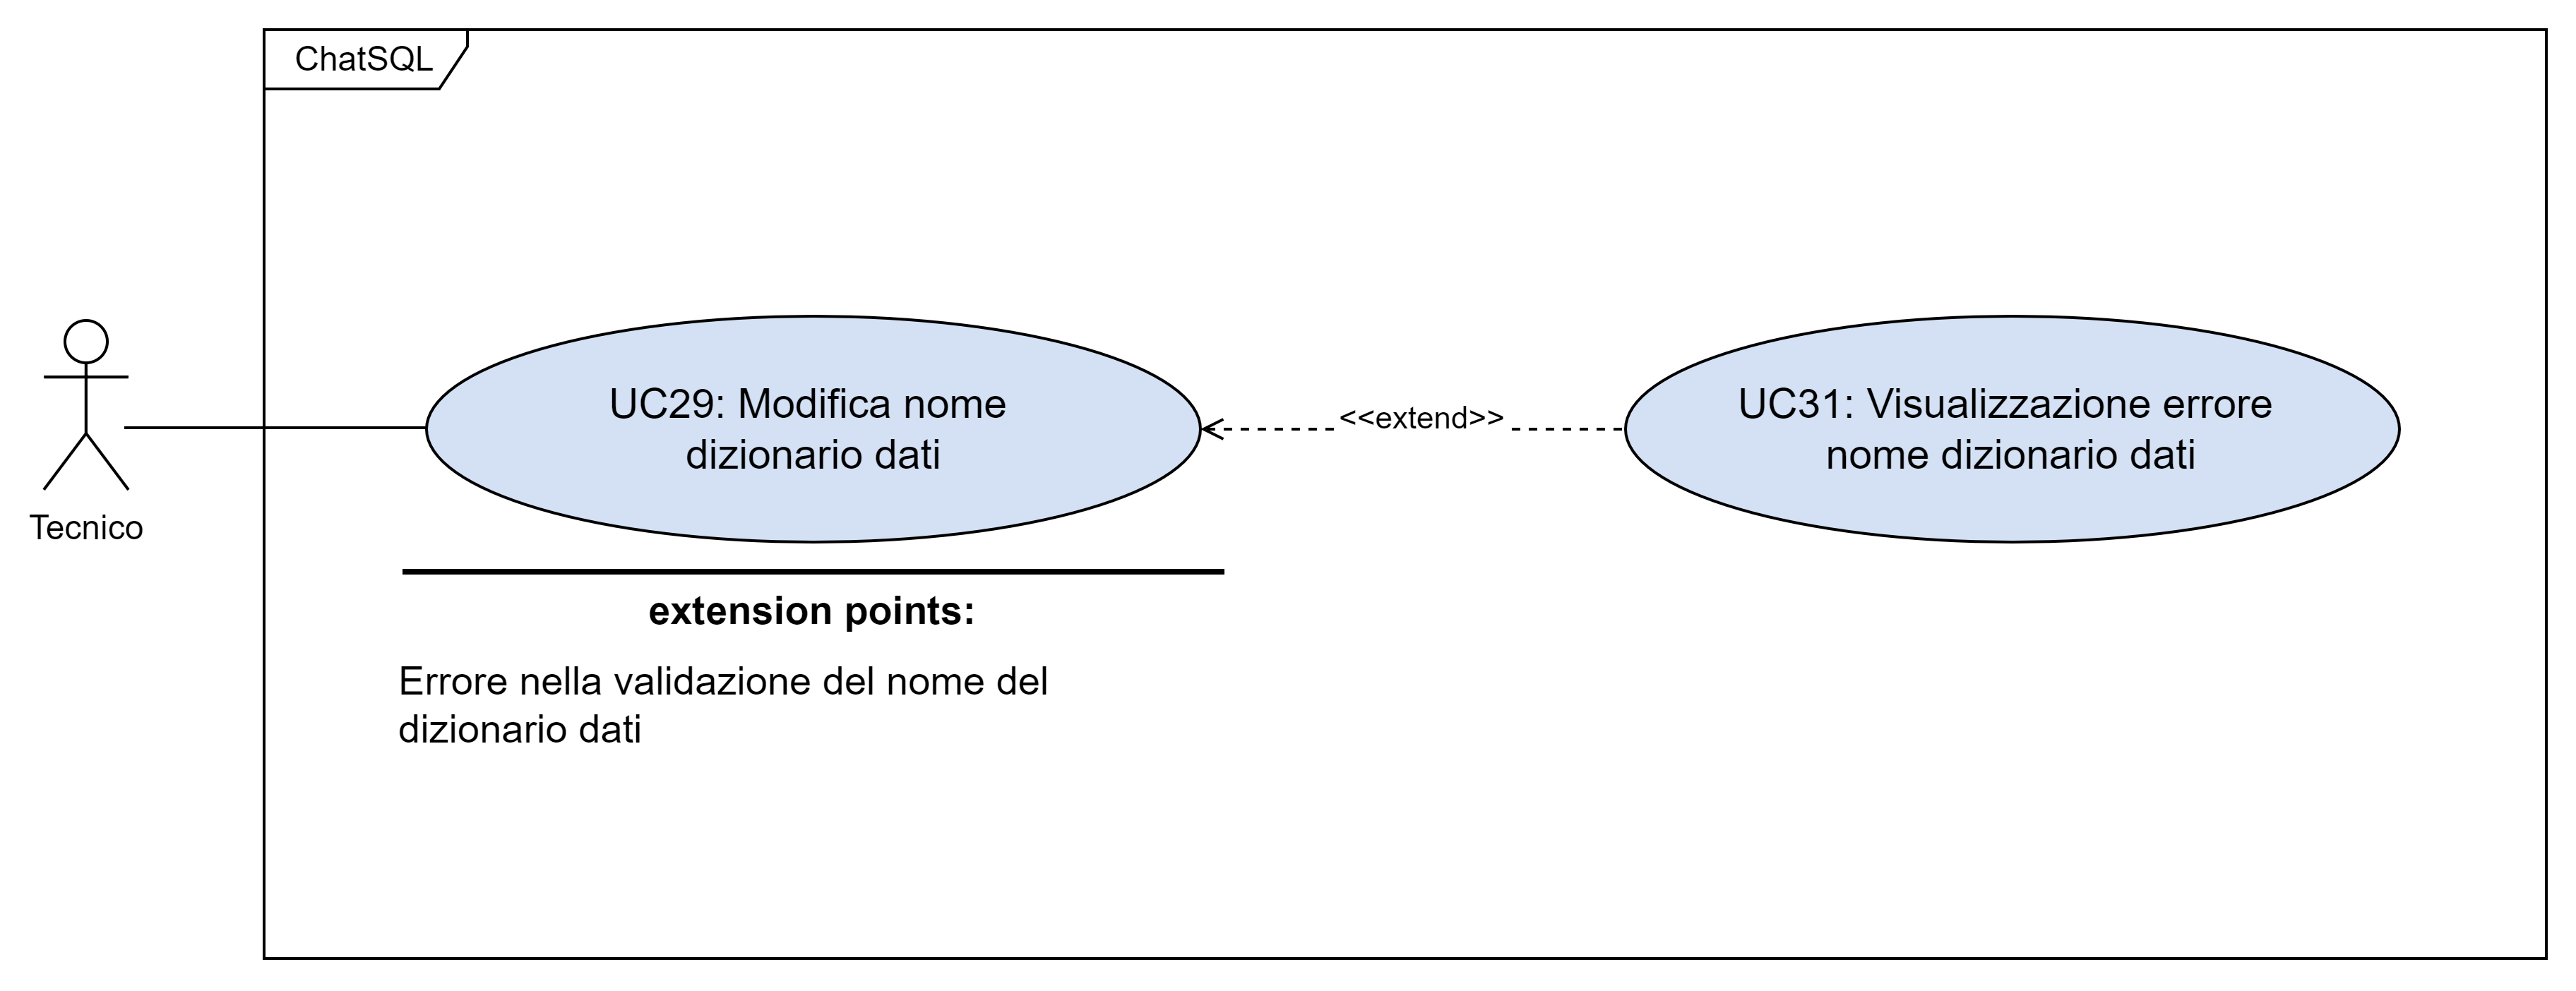
\includegraphics[width=0.95\textwidth]{assets/uc29.png}
  \caption{UC29}
\end{figure}

\paragraph*{Descrizione}
Il Tecnico modifica il nome di un \glossario{dizionario dati}.

\paragraph*{Attori principali}
Tecnico

\paragraph*{Precondizioni}
\begin{itemize}
  \item Il sistema è attivo e funzionante;
  \item Il Tecnico ha effettuato l'autenticazione (\hyperref[UC1]{UC1});
  \item Il Tecnico ha visualizzato la lista dei \glossario{dizionari dati} (\hyperref[UC9]{UC9});
  \item Il Tecnico ha individuato il dizionario da modificare (\hyperref[UC9.1]{UC9.1}).
\end{itemize}

\paragraph*{Postcondizioni}
\begin{itemize}
  \item Il nome del \glossario{dizionario dati} è stato modificato correttamente.
\end{itemize}

\paragraph*{Trigger}
Il Tecnico vuole modificare il nome di un \glossario{dizionario dati}.

\paragraph*{Scenario principale}
\begin{enumerate}
  \item Il Tecnico modifica il nome di un \glossario{dizionario dati};
  \item Il sistema sostituisce il nome del dizionario dati con il nuovo valore inserito dal Tecnico.
\end{enumerate}

\paragraph*{Scenario alternativo}
\begin{enumerate}
  \item Il sistema riscontra un errore durante la validazione del nome (\hyperref[UC31]{UC31});
  \item Viene visualizzato un messaggio con i dettagli dell'errore.
\end{enumerate}

\paragraph*{Estensioni}
\begin{itemize}
  \item Visualizzazione errore nome dizionario dati (\hyperref[UC31]{UC31}):
  \begin{itemize}
    \item Extension point: Errore nella validazione del nome del dizionario dati.
  \end{itemize}
\end{itemize}